\section{Experiments}\label{sec:experiments}

We now present experiments validating our optimizers.
We show that training neural networks via convex reformulations is faster and more robust than attempting to solve the non-convex training problem with SGD~\citep{robbins1951sgd} or Adam~\citep{kingma2015adam}.
Moreover, the models learned by convex optimization are consistent and generalize as well as Adam/SGD without their failure modes.

\subsection{Optimization Performance}\label{sec:optimization-performance}


\setlength{\tabcolsep}{3pt} % Default value: 6pt
\begin{table}[t]
	\centering
	\caption{Approximating the C-ReLU problem with cone decompositions.
		We compare the solution to C-GReLU (FISTA) with cone-decomposition by solving the min-norm program (CD-SOCP),
		the approximate cone decomposition (CD-A), and directly solving C-ReLU using the AL method.
		Exactly solving CD-SOCP is costly compared to direct solutions.
		Although CD-A gives only an approximate decomposition, it yields similar
		test performance to CD-SOCP and is two orders of magnitude faster.
	}%
	\label{table:cone-decomp}
	\vspace{0.1in}
	\begin{small}
		\begin{tabular}{lcccccccc}
			                 & \multicolumn{2}{c}{\textbf{R-FISTA}} & \multicolumn{2}{c}{\textbf{CD-SOCP}} & \multicolumn{2}{c}{\textbf{CD-A}} & \multicolumn{2}{c}{\textbf{AL}}                              \\ \cmidrule(lr){2-3}  \cmidrule(lr){4-5}  \cmidrule(lr){6-7} \cmidrule(lr){8-9}
			\textbf{Dataset} & Acc.                                 & Time                                 & Acc.                              & Time                            & Acc. & Time & Acc. & Time  \\ \midrule
			energy           & 86.3                                 & 0.12                                 & 86.3                              & 134.6                           & 86.3 & 1.56 & 83.7 & 5.05  \\
			ecoli            & 71.6                                 & 0.07                                 & 71.6                              & 149.7                           & 70.1 & 0.29 & 70.1 & 3.38  \\
			glass            & 64.3                                 & 0.13                                 & 64.3                              & 68.76                           & 64.3 & 0.57 & 61.9 & 3.0   \\
			pima             & 73.2                                 & 0.36                                 & 73.2                              & 37.68                           & 73.2 & 4.24 & 75.8 & 4.72  \\
			oocytes          & 78.6                                 & 0.98                                 & 79.1                              & 136.3                           & 78.0 & 4.68 & 74.2 & 81.68 \\ \bottomrule
		\end{tabular}
	\end{small}
\end{table}
\setlength{\tabcolsep}{6pt}






%% Old Tables...

\iffalse
	\begin{table}
		\begin{tabular}{lllllllllllllll}
			                                  & fista    &          &      & LP       &          &        & SOCP     &          &        & AP       &          &       &   & \\
			                                  & accuracy & norm     & time & accuracy & norm     & time   & accuracy & norm     & time   & accuracy & norm     & time  &     \\
			breast-cancer                     & 68.4     & 1.06e+02 & 0.84 & 68.4     & 2.68e+08 & 8.12   & 68.4     & 3.73e+03 & 12.14  & 66.7     & 5.84e+01 & 6.17  &   & \\
			breast-cancer-wisc-diag           & 97.3     & 4.20e+01 & 0.89 & 97.3     & 7.06e+08 & 68.61  & 97.3     & 1.90e+03 & 80.69  & 99.1     & 3.48e+01 & 18.32 &   & \\
			congressional-voting              & 64.4     & 2.25e+01 & 0.45 & 64.4     & 8.19e+03 & 21.86  & 64.4     & 1.28e+02 & 23.13  & 69.0     & 2.33e+01 & 4.34  &   & \\
			credit-approval                   & 82.6     & 7.32e+01 & 0.44 & 82.6     & 4.06e+08 & 46.02  & 83.3     & 3.97e+03 & 63.46  & 84.1     & 5.11e+01 & 6.46  &   & \\
			cylinder-bands                    & 75.5     & 9.64e+01 & 1.18 & 75.5     & 5.81e+05 & 68.44  & 77.5     & 2.09e+03 & 79.78  & 75.5     & 1.11e+02 & 15.18 &   & \\
			ecoli                             & 71.6     & 1.73e+01 & 0.07 & 71.6     & 5.02e+05 & 63.42  & 71.6     & 5.82e+02 & 149.75 & 70.1     & 1.68e+01 & 3.38  &   & \\
			energy-y1                         & 86.3     & 2.90e+01 & 0.12 & 86.3     & 4.99e+08 & 81.65  & 86.3     & 2.34e+03 & 134.54 & 83.7     & 2.89e+01 & 5.05  &   & \\
			glass                             & 64.3     & 2.00e+01 & 0.13 & 64.3     & 1.57e+05 & 31.64  & 64.3     & 4.05e+02 & 68.76  & 61.9     & 1.72e+01 & 3.0   &   & \\
			heart-cleveland                   & 51.7     & 1.97e+01 & 0.13 & 51.7     & 1.37e+05 & 60.59  & 51.7     & 2.52e+02 & 109.48 & 50.0     & 1.77e+01 & 1.82  &   & \\
			heart-hungarian                   & 86.2     & 8.01e+01 & 0.88 & 86.2     & 2.01e+08 & 11.2   & 86.2     & 2.75e+03 & 17.14  & 84.5     & 5.09e+01 & 7.01  &   & \\
			heart-va                          & 35.0     & 2.44e+01 & 0.16 & 35.0     & 4.79e+08 & 32.62  & 37.5     & 4.79e+02 & 67.11  & 37.5     & 1.58e+01 & 1.86  &   & \\
			hepatitis                         & 80.6     & 2.96e+01 & 1.06 & 80.6     & 5.50e+04 & 7.84   & 80.6     & 2.63e+02 & 10.57  & 74.2     & 5.53e+01 & 8.56  &   & \\
			horse-colic                       & 85.0     & 5.79e+01 & 1.0  & 85.0     & 1.84e+05 & 23.33  & 86.7     & 9.45e+02 & 29.42  & 90.0     & 8.92e+01 & 9.75  &   & \\
			ionosphere                        & 90.0     & 4.74e+01 & 1.15 & 90.0     & 5.20e+05 & 38.34  & 90.0     & 1.51e+03 & 44.12  & 90.0     & 6.42e+01 & 15.91 &   & \\
			mammographic                      & 78.1     & 4.13e+01 & 0.24 & 77.6     & 1.23e+08 & 25.71  & 78.1     & 8.11e+03 & 33.17  & 79.2     & 3.70e+01 & 5.14  &   & \\
			monks-2                           & 60.6     & 1.02e+02 & 1.95 & 63.6     & 3.45e+08 & 3.98   & 60.6     & 7.36e+03 & 5.81   & 45.5     & 8.13e+01 & 18.31 &   & \\
			monks-3                           & 87.5     & 5.59e+01 & 1.6  & 87.5     & 1.29e+08 & 2.84   & 87.5     & 3.44e+03 & 3.89   & 95.8     & 8.60e+01 & 31.84 &   & \\
			oocytes\_trisopterus\_nucleus\_2f & 78.6     & 1.14e+02 & 0.98 & 66.5     & 7.51e+11 & 118.59 & 79.1     & 1.19e+04 & 136.33 & 74.2     & 8.54e+01 & 81.68 &   & \\
			parkinsons                        & 92.3     & 4.70e+01 & 1.9  & 87.2     & 6.44e+07 & 13.0   & 92.3     & 1.06e+03 & 16.0   & 89.7     & 6.69e+01 & 19.04 &   & \\
			pima                              & 73.2     & 7.88e+01 & 0.36 & 73.2     & 5.94e+05 & 29.19  & 73.2     & 8.09e+03 & 37.68  & 75.8     & 4.03e+01 & 4.72  &   & \\
			planning                          & 63.9     & 8.94e+01 & 1.33 & 63.9     & 5.85e+08 & 6.74   & 63.9     & 2.16e+03 & 10.54  & 58.3     & 1.09e+02 & 9.74  &   & \\
			seeds                             & 95.2     & 1.91e+01 & 0.25 & 95.2     & 1.09e+05 & 12.04  & 95.2     & 4.83e+02 & 26.71  & 95.2     & 1.82e+01 & 5.16  &   & \\
			statlog-australian-credit         & 64.5     & 1.58e+02 & 0.69 & 63.8     & 2.96e+08 & 42.92  & 63.8     & 1.06e+04 & 55.59  & 65.2     & 2.74e+01 & 4.8   &   & \\
			statlog-heart                     & 81.5     & 6.76e+01 & 0.81 & 81.5     & 3.65e+08 & 10.63  & 81.5     & 1.48e+03 & 15.57  & 85.2     & 6.11e+01 & 7.36  &   & \\
			teaching                          & 40.0     & 3.71e+01 & 0.24 & 40.0     & 3.27e+05 & 5.88   & 40.0     & 1.10e+03 & 12.18  & 33.3     & 2.21e+01 & 2.05  &   & \\
			tic-tac-toe                       & 97.9     & 1.70e+02 & 0.45 & 97.9     & 2.65e+05 & 46.69  & 97.9     & 6.86e+03 & 60.36  & 93.7     & 1.57e+02 & 14.25 &   & \\
			vertebral-column-2clases          & 88.7     & 7.41e+01 & 0.68 & 88.7     & 1.23e+10 & 6.25   & 88.7     & 7.76e+03 & 9.64   & 90.3     & 4.74e+01 & 8.23  &   & \\
			wine                              & 100.0    & 1.87e+01 & 0.25 & 100.0    & 5.05e+04 & 18.03  & 100.0    & 1.97e+02 & 32.05  & 100.0    & 1.78e+01 & 3.67  &   &
		\end{tabular}
	\end{table}


	\begin{table*}[t]
		\centering
		\begin{tabular}{lcccccccccccc} \toprule
			                 & \multicolumn{3}{c}{C-GReLU} & \multicolumn{3}{c}{C-GReLU + LP} & \multicolumn{3}{c}{C-GReLU + COCP} & \multicolumn{3}{c}{C-ReLU}                                                                                   \\ \cmidrule(lr){2-4}  \cmidrule(lr){5-7}  \cmidrule(lr){8-10} \cmidrule(lr){11-13}
			\textbf{Dataset} & Acc.                        & Norm                             & Time                               & Acc.                       & Norm     & Time     & Acc.  & Norm     & Time     & Acc.  & Norm     & Time     \\ \midrule
			breast-cancer    & 68.4                        & 1.06e+02                         & 8.39e-01                           & 68.4                       & 2.68e+08 & 8.12e+00 & 68.4  & 3.73e+03 & 1.21e+01 & 66.7  & 5.84e+01 & 6.17e+00 \\
			congressional    & 64.4                        & 2.25e+01                         & 4.52e-01                           & 64.4                       & 8.19e+03 & 2.19e+01 & 64.4  & 1.28e+02 & 2.31e+01 & 69.0  & 2.33e+01 & 4.34e+00 \\
			sonar            & 87.8                        & 2.48e+01                         & 1.44e+00                           & 87.8                       & 7.30e+04 & 3.70e+01 & 90.2  & 2.29e+02 & 4.00e+01 & 87.8  & 4.94e+01 & 1.58e+01 \\
			credit-approval  & 82.6                        & 7.32e+01                         & 4.40e-01                           & 82.6                       & 4.06e+08 & 4.60e+01 & 83.3  & 3.97e+03 & 6.35e+01 & 84.1  & 5.11e+01 & 6.46e+00 \\
			cylinder-bands   & 75.5                        & 9.64e+01                         & 1.18e+00                           & 75.5                       & 5.81e+05 & 6.84e+01 & 77.5  & 2.09e+03 & 7.98e+01 & 75.5  & 1.11e+02 & 1.52e+01 \\
			ecoli            & 71.6                        & 1.73e+01                         & 7.22e-02                           & 71.6                       & 5.02e+05 & 6.34e+01 & 71.6  & 5.82e+02 & 1.50e+02 & 70.1  & 1.68e+01 & 3.38e+00 \\
			energy-y1        & 86.3                        & 2.90e+01                         & 1.20e-01                           & 86.3                       & 4.99e+08 & 8.17e+01 & 86.3  & 2.34e+03 & 1.35e+02 & 83.7  & 2.89e+01 & 5.05e+00 \\
			glass            & 64.3                        & 2.00e+01                         & 1.26e-01                           & 64.3                       & 1.57e+05 & 3.16e+01 & 64.3  & 4.05e+02 & 6.88e+01 & 61.9  & 1.72e+01 & 3.00e+00 \\
			cleveland        & 51.7                        & 1.97e+01                         & 1.34e-01                           & 51.7                       & 1.37e+05 & 6.06e+01 & 51.7  & 2.52e+02 & 1.09e+02 & 50.0  & 1.77e+01 & 1.82e+00 \\
			hungarian        & 86.2                        & 8.01e+01                         & 8.77e-01                           & 86.2                       & 2.01e+08 & 1.12e+01 & 86.2  & 2.75e+03 & 1.71e+01 & 84.5  & 5.09e+01 & 7.01e+00 \\
			heart-va         & 35.0                        & 2.44e+01                         & 1.61e-01                           & 35.0                       & 4.79e+08 & 3.26e+01 & 37.5  & 4.79e+02 & 6.71e+01 & 37.5  & 1.58e+01 & 1.86e+00 \\
			hepatitis        & 80.6                        & 2.96e+01                         & 1.06e+00                           & 80.6                       & 5.50e+04 & 7.84e+00 & 80.6  & 2.63e+02 & 1.06e+01 & 74.2  & 5.53e+01 & 8.56e+00 \\
			horse-colic      & 85.0                        & 5.79e+01                         & 1.00e+00                           & 85.0                       & 1.84e+05 & 2.33e+01 & 86.7  & 9.45e+02 & 2.94e+01 & 90.0  & 8.92e+01 & 9.75e+00 \\
			ionosphere       & 90.0                        & 4.74e+01                         & 1.15e+00                           & 90.0                       & 5.20e+05 & 3.83e+01 & 90.0  & 1.51e+03 & 4.41e+01 & 90.0  & 6.42e+01 & 1.59e+01 \\
			mammographic     & 78.1                        & 4.13e+01                         & 2.40e-01                           & 77.6                       & 1.23e+08 & 2.57e+01 & 78.1  & 8.11e+03 & 3.32e+01 & 79.2  & 3.70e+01 & 5.14e+00 \\
			monks-2          & 60.6                        & 1.02e+02                         & 1.95e+00                           & 63.6                       & 3.45e+08 & 3.98e+00 & 60.6  & 7.36e+03 & 5.81e+00 & 45.5  & 8.13e+01 & 1.83e+01 \\
			monks-3          & 87.5                        & 5.59e+01                         & 1.60e+00                           & 87.5                       & 1.29e+08 & 2.84e+00 & 87.5  & 3.44e+03 & 3.89e+00 & 95.8  & 8.60e+01 & 3.18e+01 \\
			oocytes          & 78.6                        & 1.14e+02                         & 9.84e-01                           & 66.5                       & 7.51e+11 & 1.19e+02 & 79.1  & 1.19e+04 & 1.36e+02 & 74.2  & 8.54e+01 & 8.17e+01 \\
			parkinsons       & 92.3                        & 4.70e+01                         & 1.90e+00                           & 87.2                       & 6.44e+07 & 1.30e+01 & 92.3  & 1.06e+03 & 1.60e+01 & 89.7  & 6.69e+01 & 1.90e+01 \\
			pima             & 73.2                        & 7.88e+01                         & 3.58e-01                           & 73.2                       & 5.94e+05 & 2.92e+01 & 73.2  & 8.09e+03 & 3.77e+01 & 75.8  & 4.03e+01 & 4.72e+00 \\
			planning         & 63.9                        & 8.94e+01                         & 1.33e+00                           & 63.9                       & 5.85e+08 & 6.74e+00 & 63.9  & 2.16e+03 & 1.05e+01 & 58.3  & 1.09e+02 & 9.74e+00 \\
			seeds            & 95.2                        & 1.91e+01                         & 2.54e-01                           & 95.2                       & 1.09e+05 & 1.20e+01 & 95.2  & 4.83e+02 & 2.67e+01 & 95.2  & 1.82e+01 & 5.16e+00 \\
			australian       & 64.5                        & 1.58e+02                         & 6.87e-01                           & 63.8                       & 2.96e+08 & 4.29e+01 & 63.8  & 1.06e+04 & 5.56e+01 & 65.2  & 2.74e+01 & 4.80e+00 \\
			statlog-heart    & 81.5                        & 6.76e+01                         & 8.08e-01                           & 81.5                       & 3.65e+08 & 1.06e+01 & 81.5  & 1.48e+03 & 1.56e+01 & 85.2  & 6.11e+01 & 7.36e+00 \\
			teaching         & 40.0                        & 3.71e+01                         & 2.45e-01                           & 40.0                       & 3.27e+05 & 5.88e+00 & 40.0  & 1.10e+03 & 1.22e+01 & 33.3  & 2.21e+01 & 2.05e+00 \\
			tic-tac-toe      & 97.9                        & 1.70e+02                         & 4.49e-01                           & 97.9                       & 2.65e+05 & 4.67e+01 & 97.9  & 6.86e+03 & 6.04e+01 & 93.7  & 1.57e+02 & 1.43e+01 \\
			vertebral-col.   & 88.7                        & 7.41e+01                         & 6.78e-01                           & 88.7                       & 1.23e+10 & 6.25e+00 & 88.7  & 7.76e+03 & 9.64e+00 & 90.3  & 4.74e+01 & 8.23e+00 \\
			wine             & 100.0                       & 1.87e+01                         & 2.49e-01                           & 100.0                      & 5.05e+04 & 1.80e+01 & 100.0 & 1.97e+02 & 3.21e+01 & 100.0 & 1.78e+01 & 3.67e+00
		\end{tabular}
		\caption{}%
		\label{table:cone-decomp}
	\end{table*}
\fi


\textbf{Synthetic Classification}:
Convex-reformulations offer a stable approach to model training, especially outside of the over-parameterized setting.
To illustrate this, we create a realizable problem with \( X \sim \calN\rbr{0, \Sigma} \) and \( y = \text{sign}(h_{W_1,w_2}(X)) \), where \( h_{W_1, w_2} \) is a two-layer ReLU network with \( m = 100 \) and random Gaussian weights.
We try to recover this model with ten independent runs of SGD and compare against our AL method on the C-ReLU problem.
For C-ReLU, \( \tilde \calD \) is 100 random arrangements augmented with all activations generated while solving the non-convex problem with SGD.\footnote{This guarantees the non-convex model is in the model space of the convex program.}
\cref{fig:synthetic-classification} shows that SGD converges to sub-optimal stationary points four times, while every run of the convex solver yields a model with perfect training accuracy.
See Appendix~\ref{app:synthetic-classification} for additional results.

\textbf{Large-Scale Comparison}:
\cref{fig:performance-profiles} presents two performance profiles~\citep{dolan2002benchmarking} comparing the optimization performance of R-FISTA and our AL method to Adam, SGD, and the interior-point solver MOSEK~\citep{mosek}.
MOSEK solves the convex reformulations, while Adam and SGD solve the original non-convex problems.
The profiles aggregate performance on \( 438 \) problems generated by considering six regularization parameters for \( 73 \) datasets taken from the UCI repository~\citep{dua2019uci}.
We use the default parameters for MOSEK;
for Adam and SGD, we use a batch-size of \( 10\% \) of the data and take the \emph{best} run per-problem over a grid of seven step-sizes and three different random seeds.
See Appendix~\ref{app:performance-profiles} for details.

We make the following observations: (i) R-FISTA solves \( 50 \% \) of problems two orders of magnitude faster than Adam and SGD; (ii) MOSEK scales poorly and frequently runs out of memory despite being allocated 32GB --- \( 3 \times \) more than the other solvers; (iii) although the ReLU problem is significantly harder, the AL solver converges faster and solves \( 25\% \) more problems than the best baseline.

\begin{figure}[t]
    \centering
    \ifdefined\smallPDF
        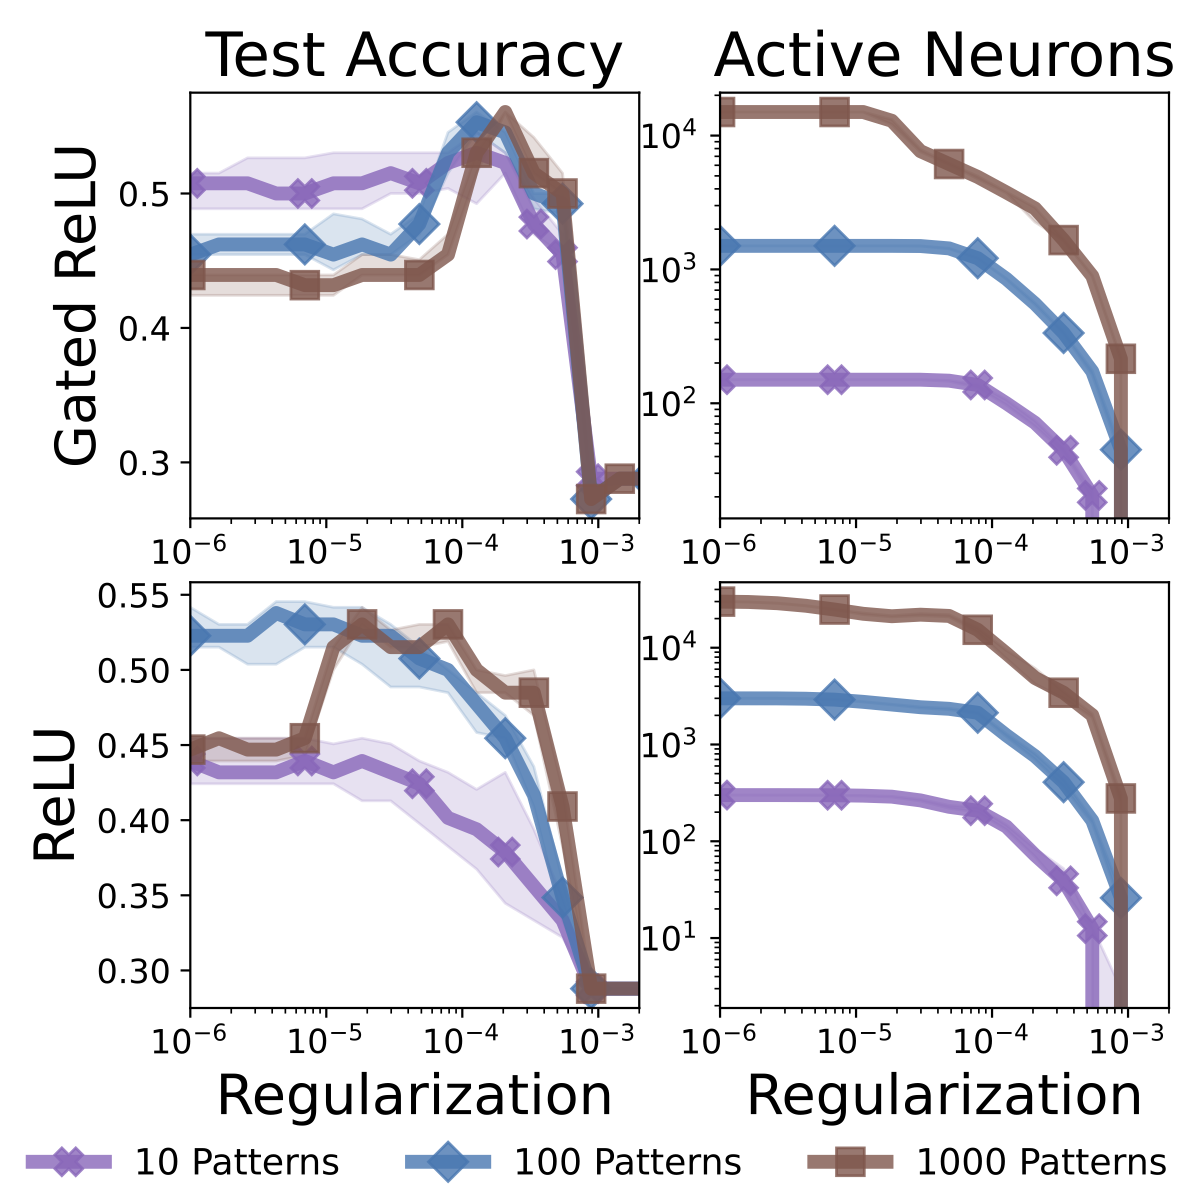
\includegraphics[width=0.98\linewidth]{figures/chapter_two/hp_paper.png}
        \vspace{-0.3cm}
    \else
        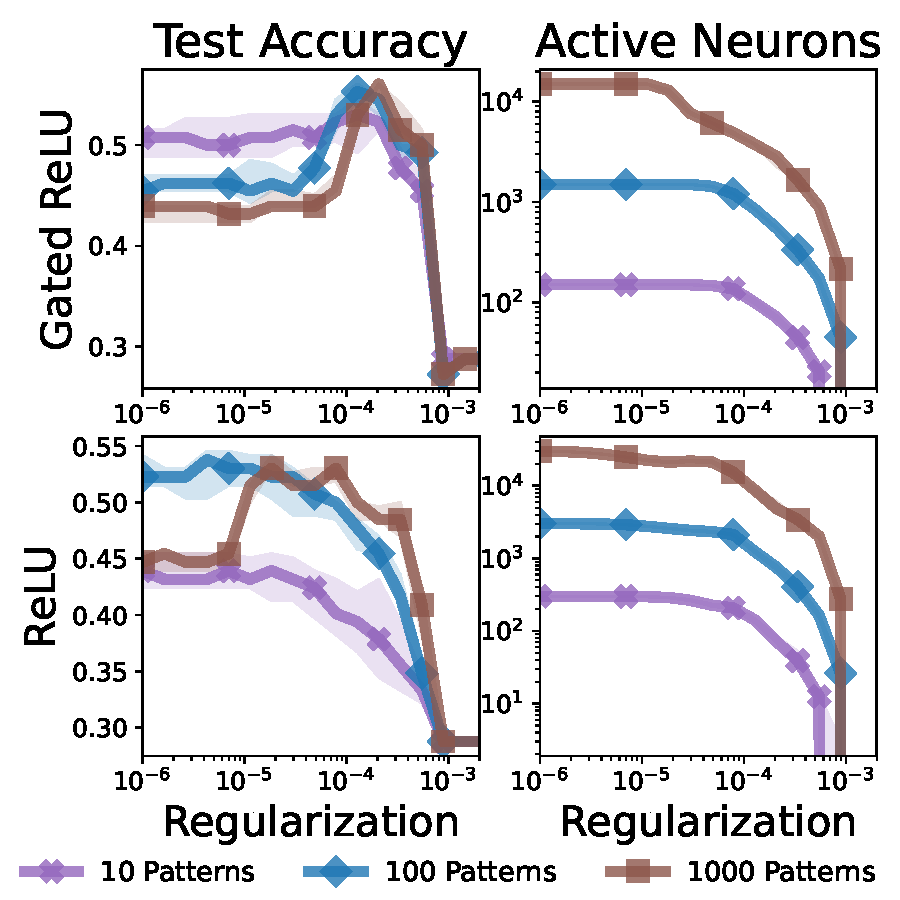
\includegraphics[width=0.98\linewidth]{figures/chapter_two/hp_paper.pdf}
        \vspace{-0.3cm}
    \fi
    \caption{
        Effect of sampling activation patterns on test accuracy for networks trained using the C-ReLU and C-GReLU problems on the \texttt{primary-tumor} dataset.
        We consider a grid of regularization parameters and plot median (solid line) and first and third quartiles (shaded region) over 10 random samplings of \( \tilde{\calD} \), where \( |\tilde{\calD}| \) is limited to 10, 100, or 1000 patterns.
    }%
    \label{fig:reg-plot}%
    \vspace{-0.3cm}
\end{figure}

\textbf{Cone Decompositions}:
We compare optimizing the C-ReLU problem directly using our AL method against \cref{alg:cone-decomp}.
We try two decomposition methods: CD-SOCP, which sets \( R(u,v) = \norm{u}_2 + \norm{v}_2 \) and solves the resulting SOCP, and
CD-A, which approximates the cone decomposition problem by solving Eq.~\eqref{eq:cd-approx}.
We use MOSEK to solve the SOCP.
\cref{table:cone-decomp} gives median test accuracy and time-to-solution for each approach on five UCI datasets.
R-FISTA is an order of magnitude faster than AL and two orders faster CD-SOCP, primarily because SOCPs must be solved on CPU.
CD-A performs comparably to CD-SOCP and is faster than solving the C-ReLU problem
with our AL method.
See \cref{app:cone-decomps} for experimental details and additional results, including model norms.

\subsection{Model Performance}\label{sec:model-performance}

\textbf{Sensitivity and Regularization}:
Figure~\ref{fig:reg-plot} shows the effects of sub-sampling activation patterns on the C-ReLU and C-GReLU problems for the \texttt{primary-tumor} dataset.
Surprisingly, we find that the distribution of test-accuracies is stable across regularization parameters even when the number of patterns is small.
We also observe an inverted-U shaped bias-variance trade-off as the regularization strength is increased, with sparse models showing the best generalization.
This contrasts the double descent phenomena frequently observed with non-convex neural networks~\citep{belkin2019reconciling, loog2020brief, nakkiran2020double}.
See Appendix~\ref{app:activation-pattern-ablations} for results on a further nine UCI datasets.

\input{results/chapter_two/binary_accuracy_table}

\textbf{UCI Classification}:
Table~\ref{table:binary-uci-accuracies} compares the performance of C-ReLU and C-GReLU
with random forests \citep{breiman2001randomforests} and SVMs \citep{boser1992svm} for binary classification on 18 UCI datsasets.
For all methods, we report test accuracy for the best hyperparameters as selected
by cross-validation.
Taken together, C-ReLU and C-GReLU perform best on 14 problems,
showing two-layer neural networks offer an effective, easy-to-train
alternative to common baselines.
Results for additional datasets are given in Appendix~\ref{app:uci-accuracies}

\textbf{Non-Convex Solvers}:
We compare the generalization of C-ReLU and C-GReLU with that of the non-convex problems on 20 UCI datasets.
For each dataset/problem, we select the regularization strength using five-fold cross validation.
For NC-ReLU and NC-GReLU, we use Adam and SGD and tune the step-sizes by cross-validation.
See Appendix~\ref{app:non-convex-solvers} for details.
Table~\ref{table:non-convex-solvers} summarizes the test accuracy results.
We find that our convex programs generalize as well as the non-convex baselines for a fraction of the training time.

\begin{table}[t]
	\centering
	\caption{Median test accuracies from five restarts on a subset of the UCI datasets.
		Results are presented as \texttt{Gated ReLU} / \texttt{ReLU}.
		Overall, we find the convex reformulations have comparable generalization to the non-convex networks.
		Note the catastrophic failure of SGD on \texttt{ecoli}.
		See Appendix~\ref{app:non-convex-solvers} for quartiles.}%
	\label{table:non-convex-solvers}
	\vspace{0.1in}
	\begin{small}
		\begin{tabular}{lccc} \toprule
			\textbf{Dataset} & \textbf{Convex} & \textbf{Adam} & \textbf{SGD} \\ \midrule
			magic            & 86.9  / 85.9    & 82.9 / 86.9   & 82.1 / 86.4  \\
			statlog-heart    & 79.6  / 83.3    & 85.2 / 83.3   & 83.3 / 79.6  \\
			mushroom         & 100 / 100       & 97.6 / 100    & 96.9 / 99.9  \\
			vertebral-col.   & 87.1  / 90.3    & 90.3 / 90.3   & 90.3 / 88.7  \\
			cardiotocogr.    & 90.1  / 89.9    & 85.6 / 36.5   & 85.2 / 88.9  \\
			abalone          & 63.8  / 66.2    & 58.7 / 65.3   & 58.1 / 66.1  \\
			annealing        & 90.6  / 90.6    & 86.2 / 93.7   & 86.2 / 88.7  \\
			car              & 89.9  / 87.8    & 83.8 / 94.8   & 83.2 / 90.1  \\
			bank             & 89.8  / 89.8    & 89.9 / 90.8   & 89.8 / 90.5  \\
			breast-cancer    & 68.4  / 68.4    & 68.4 / 64.9   & 70.2 / 68.4  \\
			page-blocks      & 96.8  / 94.0    & 92.1 / 97.1   & 92.4 / 96.9  \\
			contrac          & 45.9  / 55.1    & 53.1 / 54.4   & 53.4 / 53.7  \\
			congressional    & 63.2  / 63.2    & 64.4 / 62.1   & 66.7 / 67.8  \\
			spambase         & 93.4  / 93.3    & 91.6 / 93.5   & 91.2 / 93.2  \\
			synthetic        & 97.5  / 98.3    & 98.3 / 96.7   & 97.5 / 96.7  \\
			musk-1           & 93.7  / 93.7    & 93.7 / 96.8   & 94.7 / 95.8  \\
			ringnorm         & 69.8  / 77.0    & 77.0 / 77.3   & 77.2 / 77.4  \\
			ecoli            & 82.1  / 80.6    & 79.1 / 82.1   & 4.5  / 80.6  \\
			monks-2          & 69.7  / 69.7    & 66.7 / 69.7   & 60.6 / 72.7  \\
			hill-valley      & 62.0  / 65.3    & 57.0 / 62.8   & 58.7 / 55.4  \\ \bottomrule
		\end{tabular}
	\end{small}
\end{table}


\textbf{Image Classification:}
We study the generalization performance of the Gated ReLU model for image classification on the MNIST and CIFAR-10 datasets \citep{lecun1998gradient, krizhevsky2009learning}.
We compare R-FISTA for C-GReLU to solving the NC-GReLU problem with SGD, Adam, and Adagrad~\citep{duchi2011adagrad}.
We choose the regularization strength and step sizes for each dataset-method pair using a train/validation split (see Appendix~\ref{app:image-datasets}).
Table~\ref{table:image-datasets} shows that R-FISTA scales well to these large-scale experiments, with generalization comparable with the non-convex solvers.
This reflects our theory, which shows that these methods are fundamentally solving the same problem.

%Both datasets are composed of images with 10 classes, which we predict with a two-layer fully-connected gated ReLU network applied to the flattened representations of the input images, using one-vs-all classification when solved with our convex programs (see Appendix~\ref{app:image-datasets-theory}).

\begin{table}
	\centering
	\caption{Test accuracy of R-FISTA for the C-GReLU problem compared to SGMs for NC-GReLU on two image classification tasks.
		Models trained using the convex program have comparable test accuracy to the non-convex formulation on MNIST and are slightly better on CIFAR-10.
	}%
	\label{table:image-datasets}%
	\vspace{0.1in}
	\begin{small}
		\begin{tabular}{lcccc} \toprule
			\textbf{Dataset} & \textbf{Convex} & \textbf{Adam} & \textbf{SGD} & \textbf{Adagrad} \\ \midrule
			MNIST            & 97.6            & 98.0          & 97.2         & 97.5             \\
			CIFAR-10         & 56.4            & 50.1          & 54.3         & 54.2             \\\bottomrule
		\end{tabular}
	\end{small}
\end{table}


% \begin{table*}
%     \centering
% 	\begin{tabular}{lcccc} \toprule
% 		\textbf{Dataset}     & \textbf{Convex}  & \textbf{Adam}    & \textbf{SGD} & \textbf{Adagrad} \\ \midrule
% 		MNIST                & 97.6 & 96.5/11.0 & 96.4/97.2 & 97.0/97.5\\
% 		CIFAR-10            &  56.4 & 51.9/44.4 & 56.4/53.6  & 55.7/53.9 \\\bottomrule
% 	\end{tabular}
% 	\caption{Something something caption}%
% 	\label{table:image-datasets}
% \end{table*}


\subsection{Additional Experiments}\label{sec:additional-experiments}

We defer additional experiments to the supplementary material due to space constraints.
In Appendix~\ref{app:acceleration-exps}, we study the effects of acceleration, restarts, and line-search on the performance of the R-FISTA method and conclude that all three components are key to the efficiency of the optimization procedure.
Appendix~\ref{app:step-size-initialization} presents an ablation study for the step-size initialization procedure in R-FISTA, which is shown to be robust to the choice of \( c \).
Similarly, Appendix~\ref{app:delta-heuristic-exps} examines the windowing heuristic for the penalty strength in our AL method and shows the strategy is comparable to the best fixed \( \delta \) found by grid search.

%Finally, we present experiments on an ``active-set'' strategy where \( \tilde \calD \) is augmented with the patterns generated by training a fixed, non-convex ReLU model with a SGM.
%This strategy, which was used \cref{fig:synthetic-classification}, guarantees that solving C-ReLU leads to a lower objective value than that of NC-ReLU.
%Empirically, we observe that it can also improve model test performance.
